 \subsection{Results}

\Cref{fig:results:omp} shows the speedups obtained with the two optimized sequential versions parallelized using OpenMP, for different numbers of threads.

It is clear to see that the \soa version obtained the best results. Even considering the speedup obtained compared to the sequential \aos version, this approach to the structures implementation scales better, allowing to take further advantage of the hardware resources.

The best results were obtained using 12 threads, which in SeARCH Group Hex nodes represents the full hardware support, disregarding \intel Hyperthreading technology. While this allows two threads to run in the same processor core, it rarely is benefitial for the program execution.

\begin{figure}[!htp]
	\centering
	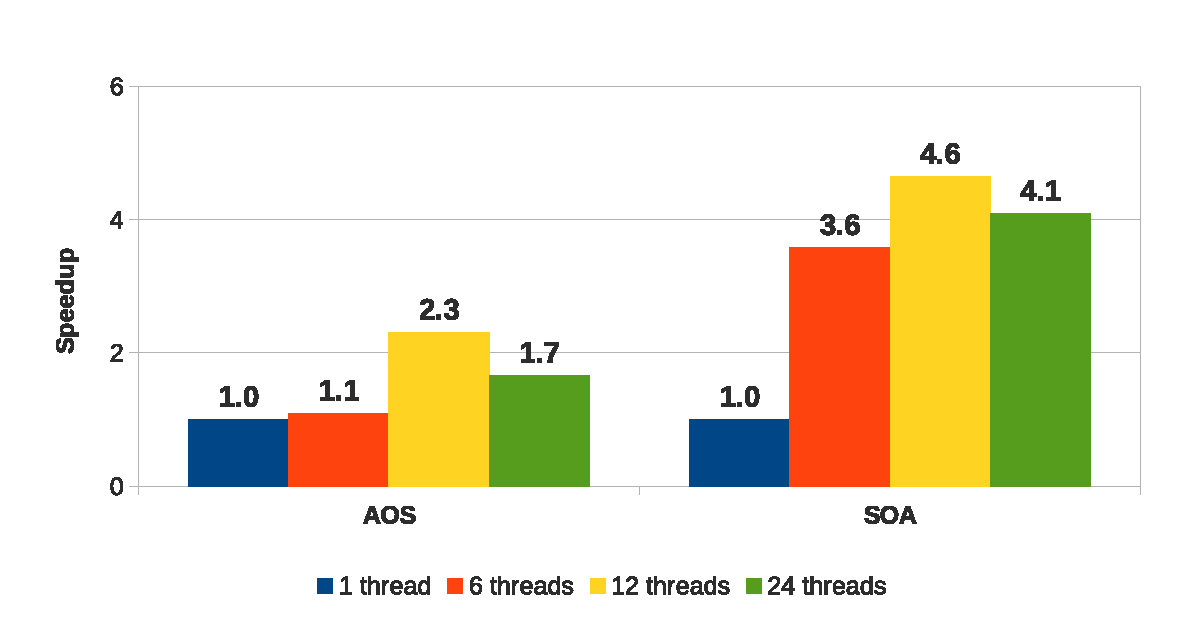
\includegraphics[width=\columnwidth]{images/graph_comparison_omp.eps}
	\caption{Speedup results for the two optimized sequential versions, parallelized with OpenMP. Original implementation used as reference.}
	\label{fig:results:omp}
\end{figure}